\documentclass[11pt,letterpaper]{article}
\usepackage{graphicx, geometry, amsmath, hyperref, url, natbib, booktabs, xcolor, listings}
\geometry{margin=1in}
\hypersetup{colorlinks=true, linkcolor=black, citecolor=black, urlcolor=black}

\title{An English Keyword Objective Is Blind to Its Own Edit in Slovene}
\author{}
\date{}

\begin{document}
\maketitle

\begin{abstract}
Abliteration removes refusal behaviour from language models by orthogonalising weights against a refusal direction extracted from English contrast pairs. The optimiser verifies candidates with an English keyword counter. We evaluate this pipeline on two 12B-parameter models---Gemma-3-12B-IT and its Slovene continual-pretraining variant GaMS3-12B-Instruct---using the RefusEU benchmark, and find that the keyword objective is structurally blind to its own edit in Slovene. Neither search reached the primary selection rule ($\leq 10/100$ keyword refusals); every candidate that a reference judge places below the selection threshold is invisible to the keyword objective (threshold-blind fraction 1.0). The keyword counter fires on 87\% of English responses but on 0\% of Slovene responses, while the reference judge finds 13\% English refusal and 82\% Slovene refusal ($\Delta_{\mathrm{lang}} = -1.56$, 95\% CI $[-1.68, -1.44]$). Keyword-verified abliterated checkpoints are therefore not valid language-neutral references for refusal evaluation. The underlying edit itself transfers asymmetrically: GaMS3 Slovene refusal drops from 87\% to 0\%, but Gemma Slovene refusal drops only from 94\% to 74\%. In a secondary analysis, depth placement of edits across layers correlates strongly with residual refusal within each model but does not transfer across architectures (Gemma vs.\ Qwen3-8B). These results are preliminary: the Slovene judge does not meet the certification gate ($\kappa = 0.72$), and 94--95\% of edited English outputs were truncated at the 256-token generation limit.
\end{abstract}

\section{Introduction}

Refusal---the learned tendency of an instruction-tuned language model to decline harmful requests---is a central component of alignment \citep{Inan2023}. Abliteration removes this behaviour by identifying a ``refusal direction'' in activation space and orthogonalising the model's weight matrices against it \citep{Arditi2024}. The refusal direction is extracted from English contrast pairs, and the optimiser (typically Heretic, a TPE-based search \citep{Akiba2019}) evaluates candidates using an English keyword counter. This pipeline has been shown to effectively suppress refusal in English, but its cross-lingual behaviour has received little attention.

The question is practically important. Open-weight models are increasingly adapted to non-English languages through continual pretraining \citep{Vres2026}, and abliterated checkpoints are widely redistributed as references for downstream safety evaluation. If the English keyword counter used to verify these checkpoints is structurally blind to non-English refusals, the checkpoints cannot serve as language-neutral references, regardless of whether the underlying edit transfers.

We study this question concretely for Slovene, a mid-resource language with approximately two million speakers. We evaluate two 12B-parameter models: \texttt{google/gemma-3-12b-it} \citep{Kamath2025} and \texttt{cjvt/GaMS3-12B-Instruct} \citep{Vres2026}, a variant of the same architecture continually pretrained on Slovene. Both models are evaluated before and after Heretic-optimised abliteration, across English and Slovene prompts from the RefusEU benchmark \citep{Krasnodebska2026}. A fifth checkpoint from the community (an independently abliterated Gemma) provides a reference point.

The central finding is that the English keyword objective is structurally blind to Slovene refusals: it fires on 87\% of English responses but on 0\% of Slovene responses, and every optimiser candidate that a reference judge considers well-abliterated is invisible to the keyword counter (threshold-blind fraction 1.0). Keyword-verified checkpoints therefore carry no information about non-English refusal behaviour. The underlying edit itself transfers asymmetrically: GaMS3 Slovene refusal drops from 87\% to 0\%, but Gemma Slovene refusal drops only from 94\% to 74\%.

\paragraph{Summary of Contributions.}
\begin{itemize}
\item \textbf{Keyword measurement bias.} The English keyword counter used by Heretic is silent on Slovene text: on 100 verified Gemma-edit pairs it fires on 87\% of English responses but 0\% of Slovene responses, while the reference judge finds 82\% Slovene refusal ($\Delta_{\mathrm{lang}} = -1.56$, 95\% CI $[-1.68, -1.44]$). Among all optimiser candidates, every one placed below the selection threshold is invisible to the keyword objective (threshold-blind fraction 1.0). Counted by the keyword-based scorer C, these are 6/6 Gemma and 37/37 GaMS3 candidates; the reference judge J confirms the pattern at 5/5 and 6/6. Keyword-verified abliterated checkpoints are therefore not valid language-neutral references for refusal evaluation (Section~\ref{sec:keyword-bias}).
\item \textbf{Depth placement correlates with residual refusal within a model but not across models.} In the Gemma causal write profile, depth placement correlates with residual refusal at confirmation-level Spearman $\rho = -0.96$ (English) and $\rho = -0.83$ (Slovene). In GaMS3, the correlation is $\rho = -0.90$ (Slovene). However, these depth profiles do not transfer across architectures: the cross-model Spearman between Gemma and Qwen3-8B is $-0.009$ ($n = 21$, $p = 0.16$; Section~\ref{sec:placement}).
\end{itemize}

All Slovene results carry a measurement caveat: the workhorse judge (Qwen3-14B) does not meet the $\kappa \geq 0.80$ certification gate for Slovene (unweighted $\kappa = 0.72$; Section~\ref{sec:limitations}).

\begin{figure}[!htbp]
  \centering
  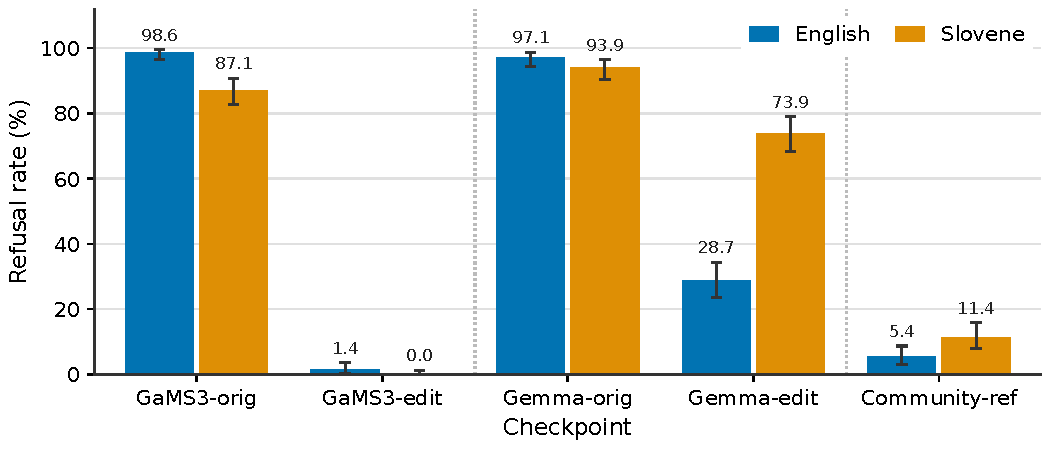
\includegraphics[width=\linewidth,height=0.85\textheight,keepaspectratio]{figures/fig_1_v0.pdf}
  \caption{Refusal rates on RefusEU S5 harmful prompts ($n=280$) for all five checkpoints in English and Slovene. Abliteration transfers almost completely to Slovene for GaMS3 (orange) but fails for Gemma (blue). The community reference checkpoint (grey) shows that deeper abliteration can partially overcome the language gap. Error bars show 95\% Clopper--Pearson confidence intervals. Note: 94--95\% of edited English outputs were truncated at the 256-token generation limit.}
  \label{fig:refusal-rates}
\end{figure}

\section{Related Work}

Representation engineering \citep{Zou2023} showed that high-level concepts, including honesty and harmfulness, are linearly represented in transformer activations. \citet{Arditi2024} extended this observation to refusal, demonstrating that a single direction in activation space mediates the refusal decision and that orthogonalising weights against this direction---abliteration---removes refusal behaviour. \citet{Wei2024} studied the brittleness of safety alignment under pruning and low-rank modifications, finding that aligned behaviour is concentrated in a small number of parameters. These results establish that refusal is geometrically localised, but none of the studies above evaluated cross-lingual transfer.

Multilingual safety evaluation has advanced through benchmarks such as RefusEU \citep{Krasnodebska2026}, which provides paired harmful and benign prompts in multiple European languages. Safety moderation tools including Llama Guard \citep{Inan2023} and PolyGuard \citep{Kumar2025} provide multilingual refusal classification. \citet{Marks2023} demonstrated that linear structure in representations generalises across domains, suggesting that refusal directions might transfer across languages. \citet{Wang2025} confirmed that a single refusal direction generalises across 14 safety-aligned languages, but evaluated the direction itself rather than the keyword-based verification that accompanies abliteration in practice. Our results partially support cross-lingual transfer for GaMS3 but not for Gemma.

Jailbreaking research \citep{Zou2023a, Shen2023, Mehrotra2023} has shown that aligned models can be attacked through adversarial suffixes, prompt injection, and automated red-teaming. \citet{Mazeika2024} introduced HarmBench as a standardised evaluation framework. Abliteration differs from these attack vectors in that it modifies the model's weights rather than its inputs, producing a permanent and deterministic change.

GaMS3 \citep{Vres2026} is a continual pretraining of Gemma-3 on 140B tokens of Slovene, English, and related South Slavic languages, followed by supervised fine-tuning on over 200K instruction examples. GlotLID \citep{Kargaran2023} provides the language identification we use to verify output language consistency.

\section{Method}

\subsection{Models and Checkpoints}

We study five checkpoints, all loaded in 4-bit NF4 quantisation throughout:
\begin{enumerate}
\item \textbf{Gemma-orig}: \texttt{google/gemma-3-12b-it} \citep{Kamath2025}, the English-centric instruction-tuned baseline.
\item \textbf{Gemma-edit}: Gemma-orig after Heretic-optimised abliteration (116 TPE trials, keyword objective). No candidate reached the primary selection rule ($\leq 10$ keyword refusals out of 100); the fallback rule selected the candidate with the lowest keyword count (72/100).
\item \textbf{GaMS3-orig}: \texttt{cjvt/GaMS3-12B-Instruct} \citep{Vres2026}, continually pretrained on Slovene.
\item \textbf{GaMS3-edit}: GaMS3-orig after Heretic-optimised abliteration (116 TPE trials, keyword objective). The fallback rule selected the candidate with the lowest keyword count (16/100).
\item \textbf{Community-ref}: An independently abliterated Gemma checkpoint from the community, included as a reference point.
\end{enumerate}

\subsection{Heretic Optimisation}

Heretic uses tree-structured Parzen estimation (TPE; \citealt{Akiba2019}) to search over abliteration hyperparameters---which layers to edit, the scaling coefficient, and the refusal-direction extraction method \citep{Arditi2024}. It optimises two objectives: an English keyword refusal rate (the fraction of 100 in-loop prompts whose responses contain English refusal keywords) and the KL divergence between the edited and original model on a calibration set. The selection rule is: minimise KL subject to refusals $\leq 10/100$; if no candidate satisfies this constraint, fall back to minimising refusals subject to KL $\leq 1.0$.

Both searches (Gemma and GaMS3) fell to the fallback branch, meaning no candidate achieved $\leq 10$ keyword refusals out of 100 in-loop prompts. The keyword objective floor (the minimum keyword refusal count across all 116 candidates) was 72 for Gemma and 16 for GaMS3.

\subsection{Evaluation Protocol}

All checkpoints are evaluated on the RefusEU benchmark \citep{Krasnodebska2026}, which provides 280 harmful prompts (S5 split) and 150 benign prompts (S6 split), each in English and Slovene. Each prompt produces a single greedy-decoded response (temperature 0, max 256 tokens). Responses are classified into \{refused, partial, complied\} by a local Qwen3-14B judge.

Refusal rate is the fraction of harmful-prompt responses classified as refused. Attack success rate (ASR) is computed over the subset of responses where both safety guards (Llama Guard 3 \citep{Inan2023} and PolyGuard \citep{Kumar2025}) agree on a label, excluding disagreements. Over-refusal rate is the fraction of benign-prompt responses classified as refused. Language consistency is verified by GlotLID \citep{Kargaran2023}.

\paragraph{Generation truncation.} The 256-token generation limit truncates a large share of edited English outputs: 95.4\% of Gemma-edit EN and 94.2\% of GaMS3-edit EN responses are truncated, compared with 96.7\% for Gemma-orig EN and 26.3\% for GaMS3-orig EN. Slovene truncation rates are lower (69.8\% for Gemma-edit SL, 92.1\% for GaMS3-edit SL). The high English truncation rate means that many compliant English responses were cut short, and the judge classified their refusal status from incomplete text.

\paragraph{Judge certification.} The Qwen3-14B workhorse judge was calibrated against GPT-4.1 labels on a held-out panel. English certification passed: unweighted $\kappa = 0.86$ $[0.77, 0.92]$, gate met. Slovene certification failed: unweighted $\kappa = 0.72$ $[0.63, 0.81]$, below the $0.80$ threshold. All Slovene absolute rates therefore carry a measurement caveat. Relative comparisons within Slovene (e.g., orig vs.\ edit) are less affected, since the judge bias is approximately constant across checkpoints.

\section{Results}
\label{sec:results}

\subsection{Refusal Suppression Across Languages}

Table~\ref{tab:headline} and Figure~\ref{fig:refusal-rates} report the main refusal evaluation. Abliteration produces dramatically different cross-lingual outcomes for the two models.

\begin{table}[!htbp]
\centering
\small
\caption{Refusal rate and attack success rate (ASR) on RefusEU S5 harmful prompts ($n=280$ per cell), with 95\% Clopper--Pearson confidence intervals. Over-refusal is on S6 benign prompts ($n=150$). Edited English outputs are truncated at 256 tokens in 94--95\% of cases (see Method).}
\label{tab:headline}
\begin{tabular}{llccc}
\toprule
Checkpoint & Lang & Refusal & ASR & Over-refusal \\
\midrule
GaMS3-orig & EN & .986 [.971,.996] & .015 [.004,.030] & .100 [.053,.153] \\
GaMS3-orig & SL & .871 [.829,.907] & .012 [.000,.027] & .107 [.060,.160] \\
GaMS3-edit & EN & .014 [.004,.029] & .982 [.964,.996] & .000 [.000,.000] \\
GaMS3-edit & SL & .000 [.000,.000] & .972 [.952,.992] & .000 [.000,.000] \\
\midrule
Gemma-orig & EN & .971 [.950,.989] & .026 [.007,.049] & .087 [.040,.133] \\
Gemma-orig & SL & .939 [.911,.964] & .016 [.004,.031] & .327 [.253,.400] \\
Gemma-edit & EN & .287 [.233,.341] & .738 [.681,.794] & .013 [.000,.033] \\
Gemma-edit & SL & .739 [.686,.786] & .103 [.067,.143] & .193 [.133,.260] \\
\midrule
Community-ref & EN & .054 [.029,.082] & 1.00 [1.00,1.00] & .007 [.000,.020] \\
Community-ref & SL & .114 [.079,.154] & .870 [.822,.909] & .027 [.007,.053] \\
\bottomrule
\end{tabular}
\end{table}

\textbf{GaMS3}: Abliteration removes refusal almost completely in both languages. English refusal drops from 98.6\% to 1.4\% (McNemar $p < 10^{-81}$); Slovene refusal drops from 87.1\% to 0.0\% ($p < 10^{-73}$). Over-refusal also drops to zero in both languages. The edit transfers fully.

\textbf{Gemma}: Abliteration partially suppresses English refusal (97.1\% $\to$ 28.7\%, $p < 10^{-57}$) but barely affects Slovene (93.9\% $\to$ 73.9\%, $p < 10^{-15}$). The English ASR reaches only 73.8\%, far below GaMS3's 98.2\%. In Slovene, Gemma-edit's ASR is 10.3\%; the edit scarcely works.

\textbf{Community reference}: The independently abliterated Gemma achieves much lower refusal in both English (5.4\%) and Slovene (11.4\%), suggesting that a more thorough abliteration procedure can reach deeper into the refusal mechanism even for Gemma.

The keyword counter that verified both the Gemma-edit and GaMS3-edit checkpoints did not detect this divergence. Both checkpoints were selected by the same fallback rule (minimise keyword refusals), and neither reached the primary gate. The next section quantifies why.

\subsection{Keyword Measurement Bias}
\label{sec:keyword-bias}

The keyword refusal counter that Heretic uses as its primary objective counts English refusal phrases (``I cannot'', ``I'm sorry'', etc.) in model responses. This counter is structurally unable to detect Slovene refusals, which are expressed in Slovene. The consequence is not merely that the optimiser misses a signal; the verified checkpoints cannot serve as language-neutral references for refusal evaluation.

We quantify the bias using the language-gap score $\Delta_{\mathrm{lang}}$, defined as the difference between the keyword-measured refusal difference (English minus Slovene) and the reference-judge-measured refusal difference. For the Gemma-edit checkpoint on a verified subset of 100 paired S5 prompts ($n=100$, Qwen reference channel): the keyword counter fires on 87\% of English responses but on 0\% of Slovene responses, while the reference judge finds 13\% English refusal and 82\% Slovene refusal.

\begin{equation}
\Delta_{\mathrm{lang}} = -1.56 \quad [95\% \text{ CI: } -1.68, -1.44]
\end{equation}

Figure~\ref{fig:keyword-bias} illustrates the gap. This decomposes into two components. The \textbf{silence component} ($-0.87$) reflects the keyword counter's inability to detect any Slovene refusals (keyword positive rate in Slovene: 0.0). The \textbf{reference component} ($-0.69$) reflects the actual difference in refusal rates between languages as measured by the judge.

\begin{figure}[!htbp]
  \centering
  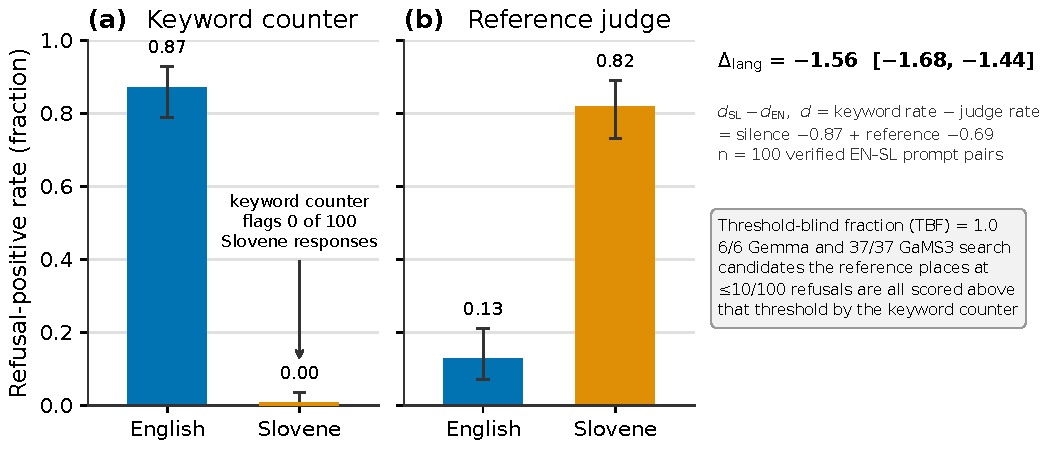
\includegraphics[width=\linewidth,height=0.85\textheight,keepaspectratio]{figures/fig_2_v0.pdf}
  \caption{Keyword counter vs.\ reference judge positive rates for the Gemma-edit checkpoint on 100 verified paired prompts. The keyword counter fires on 87\% of English responses but 0\% of Slovene responses; the reference judge finds 13\% English refusal and 82\% Slovene refusal. $\Delta_{\mathrm{lang}} = -1.56$ [$-1.68$, $-1.44$]. The keyword counter is structurally blind to Slovene refusals.}
  \label{fig:keyword-bias}
\end{figure}

The \textbf{threshold-blind fraction} (TBF) quantifies the consequence for optimiser selection. TBF is the share of candidates that a scorer places at or below the selection threshold ($\leq 10/100$ refusals) but the keyword objective places above it. In both searches, TBF $= 1.0$. Under the keyword-based scorer C, 6 out of 6 eligible Gemma candidates and 37 out of 37 eligible GaMS3 candidates are invisible to the keyword objective; under the reference judge J, the counts are 5 out of 5 and 6 out of 6. In every case the keyword counter missed every candidate that a scorer would consider well-abliterated.

Table~\ref{tab:keyword} summarises the keyword counter's behaviour across four evaluation conditions, computed on held-out prompts from both Heretic searches (first-100-token window; $n$ ranges from 70 to 490 depending on condition).

\begin{table}[!htbp]
\centering
\small
\caption{Keyword refusal counter vs.\ judge reference on held-out prompts. The keyword counter correctly identifies English refusals in unedited models (CONCORDANT) but produces zero positives on Slovene text (SILENT) and misfires on edited English text (MISFIRING, FP share 0.81).}
\label{tab:keyword}
\begin{tabular}{lccccl}
\toprule
Condition & $n$ & $\kappa$ & KW pos.\ rate & Ref.\ base rate & Mechanism \\
\midrule
Original EN & 70 & 0.20 & 0.94 & 0.94 & CONCORDANT \\
Original SL & 70 & 0.00 & 0.00 & 0.96 & SILENT \\
Edited EN & 490 & 0.02 & 0.34 & 0.17 & MISFIRING \\
Edited SL & 490 & 0.00 & 0.00 & 0.44 & SILENT \\
\bottomrule
\end{tabular}
\end{table}

The keyword counter is concordant with the judge only for unedited English models. On Slovene text, it produces zero positives regardless of whether the model actually refuses (0/490 held-out Slovene responses flagged). On edited English text, 81.4\% of its refusal detections are false positives (keyword fragments appearing in compliant responses), and its $\kappa$ against the judge is 0.02.

\subsection{Depth Placement vs.\ Dose}
\label{sec:placement}

Abliteration edits a subset of the model's transformer layers. The Heretic optimiser treats which layers to edit and the scaling coefficient as free parameters, producing candidates that vary in both \emph{where} the edit energy is placed (depth placement) and \emph{how much} total energy is applied (dose, measured as the Frobenius norm of the weight perturbation). We ask whether placement matters independently of dose.

\paragraph{Causal write profiles.} For each model, we construct a \emph{causal write profile} by applying single-layer abliteration edits to each of the model's transformer layers in isolation, then measuring the residual refusal rate. This profile reveals which layers, when edited alone, are most effective at suppressing refusal.

For Gemma, the confirmation-level Spearman correlations between the depth-placement index and residual refusal are $\rho = -0.96$ for English and $\rho = -0.83$ for Slovene ($n = 18$ weight cells). The English and Slovene profiles are correlated at $\rho = 0.59$. For GaMS3, the profile is analysed through a factorial design with two energy levels (E2 and E3) and ten placement configurations. The Spearman correlation between depth-placement index and residual Slovene refusal is $\rho = -0.90$ ($p < 10^{-7}$), holding within both energy levels ($\rho = -0.97$ at E2, $\rho = -0.95$ at E3).

\paragraph{Matched-energy contrasts.} To isolate placement from dose, we construct matched pairs of abliteration configurations that apply the same total energy across the same number of layers, but differ in which layers are edited.

Across 42 matched pairs in the Gemma experiment (energy-matched, varying layer identity), placements targeting depth-peak layers leave lower Slovene refusal than off-peak placements of equal energy (mean $\Delta_{\mathrm{SL}} = 0.12$, 95\% CI $[0.07, 0.18]$). English refusal is approximately invariant to placement at matched energy (mean $\Delta_{\mathrm{EN}} = 0.006$). Within a model, placement is a stronger predictor of Slovene refusal than dose (Figure~\ref{fig:depth-placement}).

\begin{figure}[!htbp]
  \centering
  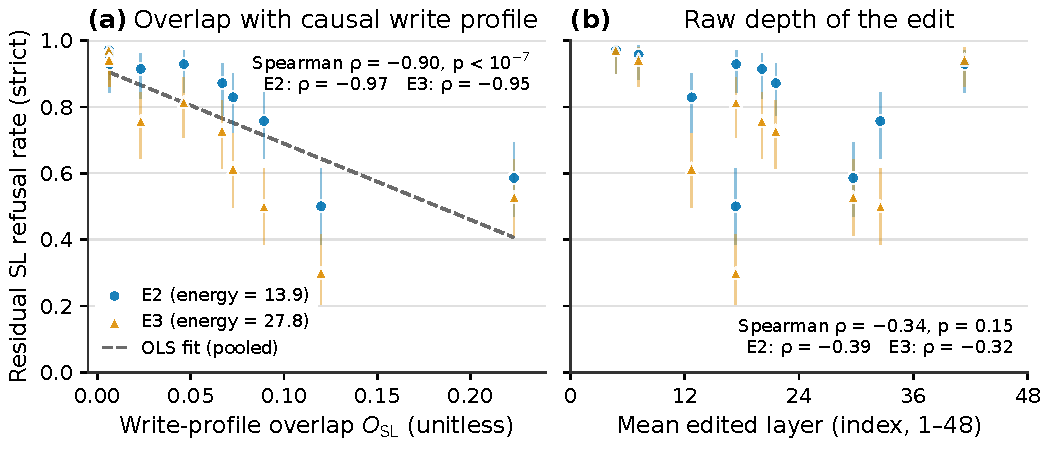
\includegraphics[width=\linewidth,height=0.85\textheight,keepaspectratio]{figures/fig_3_v0.pdf}
  \caption{Residual Slovene refusal rate as a function of depth placement for GaMS3-12B-Instruct. Each point is a single abliteration configuration; the x-axis is a depth-placement index (lower = shallower layers). Spearman $\rho = -0.90$ ($p < 10^{-7}$). Deeper placements produce lower residual Slovene refusal. The relationship holds within both energy levels (E2: $\rho = -0.97$; E3: $\rho = -0.95$).}
  \label{fig:depth-placement}
\end{figure}

\paragraph{Cross-model transfer failure.} We test whether the depth placement that works best for one model predicts what will work for another, using single-layer write profiles from Gemma and an independently constructed profile from Qwen3-8B. The activation-space depth index fails cross-model prediction entirely: Spearman $\rho = -0.009$ over 21 matched rows (item-bootstrap 95\% CI $[-0.13, 0.19]$, permutation $p = 0.16$). The depth at which abliteration is most effective is model-specific.

\section{Discussion}

\paragraph{Evaluation validity.} The keyword measurement bias is the central finding of this study. Abliterated checkpoints verified only by an English keyword counter carry no information about non-English refusal behaviour. The keyword counter detected zero Slovene refusals across all conditions (0/490 held-out Slovene responses, 0/100 verified Gemma-edit Slovene responses), and its threshold-blind fraction was 1.0 in both searches. Any downstream use of these checkpoints as language-neutral references for safety evaluation---for example, as baselines in multilingual safety benchmarks or as components in multilingual safety pipelines---inherits this validity gap.

\paragraph{Depth placement.} The depth placement finding has a narrower scope. Within a single model, the depth at which abliteration energy is applied correlates strongly with residual refusal, particularly in Slovene. But this profile does not transfer across architectures ($\rho = -0.009$ between Gemma and Qwen3-8B). The practical consequence is limited: knowing which layers matter for one model does not help with another.

\paragraph{Model divergence.} The GaMS3--Gemma contrast is striking: the edit transfers fully to GaMS3 but largely fails on Gemma. We observe this asymmetry but do not attribute it to a specific mechanism. The two checkpoints differ in their training data (GaMS3 was continually pretrained on 140B tokens including Slovene \citep{Vres2026}), but we study only two models from one architecture family, so we cannot isolate whether continual pretraining, the specific training mix, or some other factor drives the difference.

\subsection{Limitations}
\label{sec:limitations}

Several limitations constrain the scope of these findings.

\textbf{Slovene judge certification.} The Qwen3-14B workhorse judge does not meet the $\kappa \geq 0.80$ certification gate for Slovene (unweighted $\kappa = 0.72$, CI $[0.63, 0.81]$). The certification gate requires both the population-weighted and unweighted kappa to reach 0.80; the weighted kappa is 0.87, but the unweighted kappa falls short. Absolute Slovene refusal rates may be biased. Within-Slovene relative comparisons (e.g., GaMS3-orig vs.\ GaMS3-edit) are less affected, since the bias is approximately constant across checkpoints, but we cannot rule out differential bias.

\textbf{Generation truncation.} 94--95\% of edited English outputs and 70--92\% of edited Slovene outputs were truncated at the 256-token generation limit. The judge classified refusal status from incomplete text in these cases, which may affect both refusal rate and ASR estimates.

\textbf{Two models, one architecture.} We study two closely related models (Gemma and its continual-pretraining derivative). The findings may not generalise to architecturally different families (e.g., Llama, Mistral). The Qwen3-8B data in the cross-model prediction test (Section~\ref{sec:placement}) provides one additional architecture, but a systematic survey across model families is needed.

\textbf{One target language.} Slovene is a mid-resource Indo-European language. The keyword measurement bias extends to any language the keyword counter does not cover, but the degree of edit transfer failure may differ for typologically distant or extremely low-resource languages.

\textbf{NF4 quantisation.} All experiments use 4-bit NF4 quantisation. The refusal direction and abliteration behaviour may differ at full precision or other quantisation levels.

\textbf{Single Heretic configuration.} The abliteration uses a single Heretic configuration per model (116 TPE trials, default hyperparameter ranges). A more exhaustive search might yield different results.

\section{Conclusion}

We evaluated the cross-lingual transfer of English-tuned abliteration to Slovene on two 12B-parameter models and found that keyword-verified abliterated checkpoints are not valid language-neutral references for refusal evaluation. The English keyword counter is structurally blind to Slovene refusals ($\Delta_{\mathrm{lang}} = -1.56$, threshold-blind fraction 1.0), and the two models we tested diverge dramatically in whether the edit transfers to Slovene. Depth placement of edits across layers correlates with residual refusal within each model but does not transfer across architectures. All Slovene absolute rates carry a caveat from the uncertified workhorse judge ($\kappa = 0.72$).

\bibliographystyle{plainnat}
\bibliography{references}

\end{document}
